%%%%%%%%%%%%%%%%%%%%%%%%%%%%%%%%%%%%%%%%%%%%%%%%%%%%%%%%%%%%%%%%%%%%%%%%%%%%%%%
% Chapter 4 - Improving Cerebral Blood Flow Measurements with Multi-Exposure Speckle Imaging
%%%%%%%%%%%%%%%%%%%%%%%%%%%%%%%%%%%%%%%%%%%%%%%%%%%%%%%%%%%%%%%%%%%%%%%%%%%%%%%

\chapter{Improving Cerebral Blood Flow Measurements with Multi-Exposure Speckle Imaging} \label{ch:mesi}

While the conventional LSCI technique can provide reliable measurements of relative flow, it is incapable of quantifying absolute baseline values. This complicates the chronic study and inter-animal comparisons of blood flow dynamics because variations in imaging conditions cannot be properly accounted for by the underlying model. This has not prevented LSCI from being used to study chronic changes in flow (see Section \ref{sec:chronic_hemodynamics}), but has limited the observations to predominantly qualitative interpretations \cite{Armitage:2010ga}. The technique has also been shown to underestimate large changes in relative flow and fails to produce reliable measurements in the presence of static scatters \cite{Parthasarathy:2008el}.

Multi-exposure speckle imaging (MESI) is an extension to traditional LSCI theory that accounts for static scattering and produces a more robust estimate of $\tau_c$ using multiple camera exposure times \cite{Parthasarathy:2008el}. These improvements are achieved by accounting for the heterodyne mixing of dynamic and static scattering contributions, the non-ergodicity of light, and exposure-independent noise. The model described by Parthasarathy \textit{et al.} \cite{Parthasarathy:2008el} again relates the measured $K$ with $\tau_c$:

% Equation - MESI Equation
\begin{equation}
    \label{eq:mesi}
    \resizebox{\textwidth}{!}{$
    K(T,\tau_c) =
        \left(
        \beta\rho^2\frac{e^{-2x} - 1 + 2x}{2x^2} +
        4\beta\rho(1 - \rho)\frac{e^{-x} - 1 + x}{x^2} +
        \beta(1 - \rho)^2 +
        \nu_{ne} +
        \nu_{noise}
        \right)^{1/2}
    $}
\end{equation}

\noindent where $x = T/\tau_c$, $T$ is the camera exposure time, $\beta$ is the same normalization factor that accounts for speckle averaging effects, $\rho$ is the fraction of light that is dynamically scattered, $\nu_{ne}$ is the constant variance due to nonergodic light, and $\nu_{noise}$ is the exposure-independent instrument noise. For simplicity, $\nu_{ne}$ and $\nu_{noise}$ are typically merged into a single noise parameter ($\nu_{noise}$). Similar to Equation \ref{eq:bandyopadhyay}, this expression assumes that detected photons only experience single scattering interactions and that the underlying particle motion has a Lorentzian velocity distribution. A scaling term representing the number of average dynamic scattering events can be included with $x$ to account for multiple scattering interactions \cite{Kazmi:2015du}. In the absence of static scatterers, $\rho \to 1$ and Equation \ref{eq:mesi} simplifies to Equation \ref{eq:bandyopadhyay}, excluding the noise terms. In the presence of only static scatterers, then $\rho \to 0$ and $K$ reduces to a constant $\beta(1 - \rho)^2 + \nu_{noise}$ and is independent of exposure time. This represents the upper limit of the speckle variance ($K^2$) as $T$ approaches infinity. The lower limit as $T$ approaches 0 is $\beta + \nu_{noise}$, which can be approximated with just $\beta$ because the noise will only constitute a small percentage of the total value.

A minimum of four speckle contrast images acquired at different exposure times are necessary to fit Equation \ref{eq:mesi} for the four unknown variables ($\beta$, $\rho$, $\tau_c$, $\nu_{noise}$). In practice, 15 images spanning three decades of exposure times (50 $\mu$s - 80 ms) are typically utilized to sample as much of the underlying flow distribution as possible. The MESI model has improved the quantitative accuracy of flow measurements in controlled microfluidic environments \cite{Parthasarathy:2008el, Kazmi:2015du} and closely approximates the results of direct autocorrelation measurements \cite{Kazmi:2015ji}. The technique has enabled the chronic study of CBF across multiple animals and improved the robustness of flow deficit measurements during stroke \cite{Parthasarathy:2010vo, Kazmi:2013hp, Schrandt:2015gu}. This chapter details an upgrade to the imaging system to perform MESI and further validation of its capabilities.



%%%%%%%%%%%%%%%%%%%%%%%%%%%%%%%%%%%%%%%%%%%%%%%%%%%%%%%%%%%%%%%%%%%%%%%%%%%%%%%
% Section 4.1 - Instrumentation Modifications
%%%%%%%%%%%%%%%%%%%%%%%%%%%%%%%%%%%%%%%%%%%%%%%%%%%%%%%%%%%%%%%%%%%%%%%%%%%%%%%
\section{Instrumentation Modifications}

The instrumentation necessary for performing MESI is similar to traditional LSCI but requires precise control over both the camera exposure time and the laser intensity. Varying the exposure time alone would result in shot noise overwhelming the speckle signal at longer exposure times because of differences in intensity. However, by modulating the amplitude of the illuminating laser light, the average intensity of the images, and therefore the shot noise, can be held constant. Passive optical devices such as AOMs have historically been used to avoid the bandwidth and dynamic range limitations of direct laser diode modulation.

Figure \ref{fig:systemschematic_3} depicts the modifications made to the LSCI illumination pathway in order to perform MESI with the system. The same 685 nm laser diode (50 mW, HL6750MG, Thorlabs, Inc.) was collimated using an aspheric lens (C240TME-B, Thorlabs, Inc.) and the beam diameter was reduced to 1 mm. The light was modulated using a 100 MHz AOM (3100-125 AOM + 1110AF-AIFO-1.0 RF Driver, Gooch \& Housego) with the first order diffraction isolated and relayed to obliquely illuminate the sample. The camera was also upgraded (acA1920-155um, 1920 x 1200 pixels, Basler AG) because the previous model did not support trigger-based control of exposure duration, which is important for implementing MESI. The new camera also offered more convenient USB 3.0 connectivity, higher maximum frame rate (164 fps), lower dark noise, and increased dynamic range. While the pixel resolution was almost doubled, only a subset of the overall sensor array was used (1200 x 1000 pixels), resulting in a FOV of 3.6 x 3.0 mm.

% Figure - System Schematic (Ver. 3)
\begin{figure}
    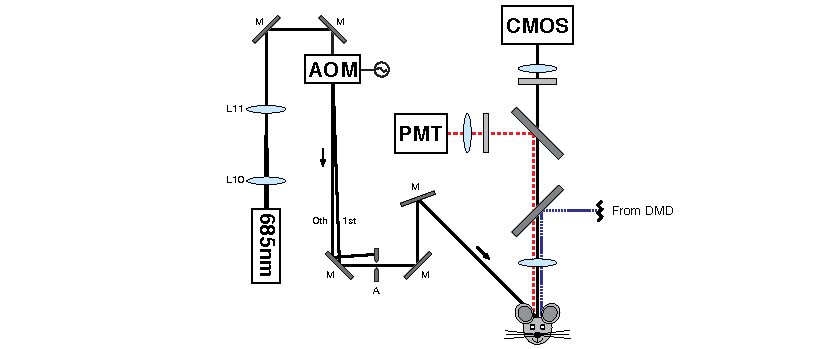
\includegraphics{figures/chapter_4/systemschematic_3.pdf}
    \caption{
        \label{fig:systemschematic_3}
        The optical system was modified to perform MESI with the addition of an AOM to modulate the 685 nm laser used for LSCI.
    }
\end{figure}

%%%%%%%%%%%%%%%%%%%%%%%%%%%%%%%%%%%%%%%%%%%%%%%%%%%%%%%%%%%%%%%%%%%%%%%%%%%%%%%
\subsection{Acquisition Control}

The MESI acquisition process is controlled by a combination of the Speckle Software and a standalone MATLAB (MathWorks, Inc.) script. The Speckle Software was updated to allow the camera to perform ``Trigger Width Exposure Mode'' acquisitions, where the duration of a hardware trigger signal directly controls the exposure time of each frame. The MATLAB script used the ANSI C NI-DAQmx library (National Instruments Corp.) to operate a multifunction I/O device (USB-6363, National Instruments Corp.) to produce the camera exposure trigger signals and AOM modulation voltages (Figure \ref{fig:mesitimingschematic}). Both waveforms were generated at 1 MHz with identical pulse durations but a slight temporal offset (+25 $\mu$s delay for the AOM signal) to guarantee that the actual camera exposures and the laser pulses were synchronized in time. This was validated using the ``Exposure Active'' output signal from the camera and a photodiode (PDA36A, Thorlabs, Inc.) directly measuring the modulated laser.

A complete MESI frame consists of 15 raw intensity images (8-bit) each acquired with a different exposure time for an effective frame rate of 2.5 fps without any averaging. This is significantly slower than standard LSCI and insufficient to properly sample faster hemodynamic processes. Because of limitations with the Speckle Software, the speckle contrast images cannot be computed for real-time visualization during an acquisition. This requires the speckle contrast images to be generated during post-processing. A standard MESI acquisition produces data at a rate of 178 MB/s.

% Figure - MESI Timing
\begin{figure}
    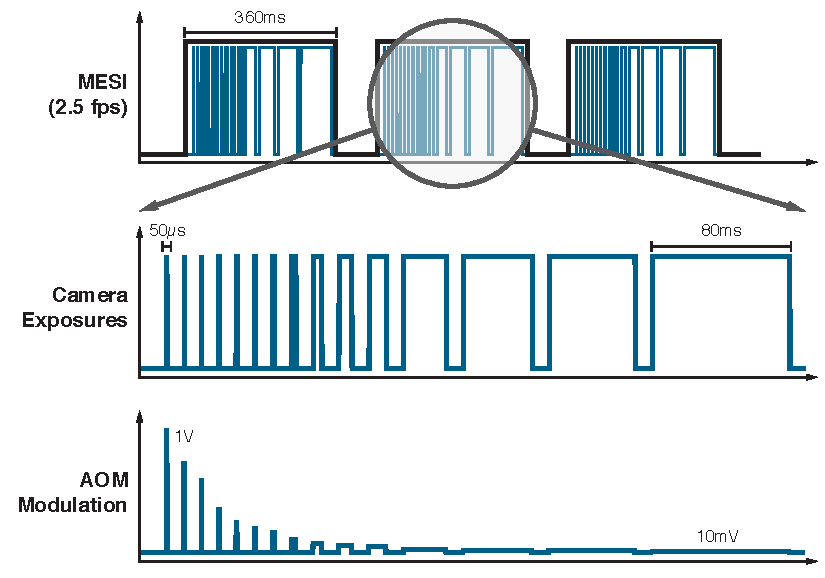
\includegraphics{figures/chapter_4/mesitimingschematic.pdf}
    \caption{
        \label{fig:mesitimingschematic}
        Timing paradigm for MESI camera exposure triggers and AOM modulation voltages. The integration of each AOM laser pulse over time is equal.
    }
\end{figure}

%%%%%%%%%%%%%%%%%%%%%%%%%%%%%%%%%%%%%%%%%%%%%%%%%%%%%%%%%%%%%%%%%%%%%%%%%%%%%%%
\subsection{Calibration Procedure}

The AOM modulation voltages for each exposure are determined using the calibration procedure outlined in Figure \ref{fig:mesicalibration}. This process ensures that shot noise is held constant across all exposures by equalizing the total amount of light used to produce each image. Because the reflectivity of the imaging surface varies by sample, the calibration must be performed prior to each MESI experiment.

% Figure - MESI Calibration
\begin{figure}
    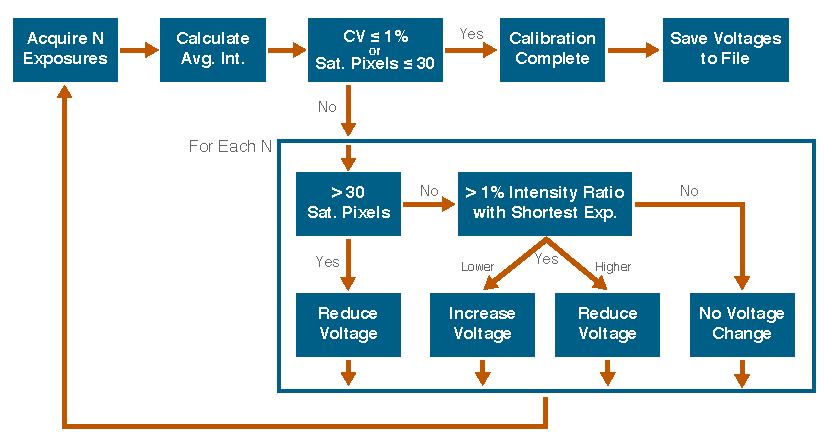
\includegraphics{figures/chapter_4/mesicalibration.pdf}
    \caption{
        \label{fig:mesicalibration}
        Overview of the MESI calibration process that attempts to equalize the raw image intensities while minimizing saturated pixels across all $N$ exposures.
    }
\end{figure}

The initial guess for the modulation voltages is generated using a power law function confined between 0-1 V. These voltages are used to acquire a complete MESI frame containing 15 raw intensity images from different exposures. The average intensity and total number of saturated pixels within a user-defined region is then calculated for each image. If the overall coefficient of variation and the number of saturated pixels are less than the defined thresholds, then the intensities are equalized and the calibration is complete. However, if the average intensity variation is too high or if there are too many saturated pixels, then each of the modulation voltages are adjusted accordingly using the shortest exposure time as the target intensity. This process repeats recursively until the stop conditions are achieved. A typical calibration will take between 30-50 iterations and complete within less than a minute.

% Figure - MESI Raw
\begin{figure}
    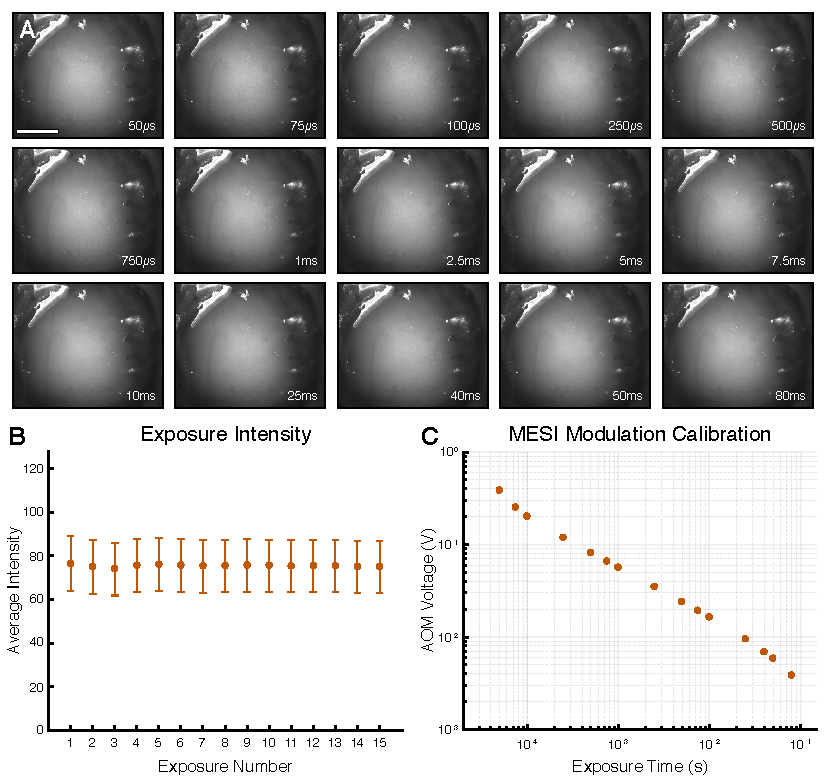
\includegraphics{figures/chapter_4/rawmesi.pdf}
    \caption{
        \label{fig:rawmesi}
        \textbf{(A)} Raw images of a cranial window from each of the 15 MESI exposures acquired using calibrated modulation voltages to equalize intensity (Scale bar = 1 mm). \textbf{(B)} Average intensity from the center quadrant of each image (mean $\pm$ s.d.). \textbf{(C)} Calibrated MESI modulation voltages for each exposure time.
    }
\end{figure}

Figure \ref{fig:rawmesi} contains an example of the final iteration of a MESI calibration for an \textit{in vivo} imaging experiment. The intensity-equalized raw images for each of the 15 exposures can be seen in Figure \ref{fig:rawmesi}A. The speckle pattern becomes increasingly blurred, especially within vascular regions, as the camera integration time increases. The average intensity from the center quadrant of each exposure is shown in Figure \ref{fig:rawmesi}B, with a final coefficient of variation \textless1\%. Figure \ref{fig:rawmesi}C depicts the resulting calibrated AOM modulation voltages for use with each exposure time during the actual imaging experiment. The voltages span two orders of magnitude (0.3 V - 3 mV) and cover the entire modulation range of the AOM.



%%%%%%%%%%%%%%%%%%%%%%%%%%%%%%%%%%%%%%%%%%%%%%%%%%%%%%%%%%%%%%%%%%%%%%%%%%%%%%%
% Section 4.2 - Improving MESI Processing Speed
%%%%%%%%%%%%%%%%%%%%%%%%%%%%%%%%%%%%%%%%%%%%%%%%%%%%%%%%%%%%%%%%%%%%%%%%%%%%%%%
\section{Improving MESI Processing Speed} \label{sec:mesi_fit}

The generation of a single MESI ICT frame is a computationally-intensive task that requires fitting Equation \ref{eq:mesi} at every single pixel of the input speckle contrast images. This has prohibited any real-time visualization using the technique and limited most studies to ROI analysis rather than full-field imagery. The original processing script developed by Parthasarthy \cite{Parthasarthy:2010uf} and improved upon by Kazmi \cite{Kazmi:2014vi} relied upon the nonlinear regression functions of MATLAB's Optimization Toolbox. The \texttt{fit()} function was used to solve for the four variables ($\beta$, $\rho$, $\tau_c$, $\nu_{noise}$) using the Trust-Region-Reflective least squares algorithm \cite{Yuan:1999tk}. This method was the only built-in algorithm that offered bound constraints on the individual components, which were necessary because all four variables are limited to values between $(0,1]$. Because the analytical Jacobian for the MESI Equation (Equation \ref{eq:mesi}) was not explicitly defined, the solver automatically approximated it using finite differences at the expense of additional computation. While this processing script produced reliable results, it was extremely slow and took hours to compute a single MESI ICT image, making it impractical to generate more than a few frames.

In order to increase the processing speed, alternatives to the native MATLAB optimization functions were examined. The Levenberg-Marquardt nonlinear least squares algorithm has a popular ANSI C implementation (\texttt{levmar}) \cite{Lourakis:J2fCMU5i} that offers interfacing with MATLAB via a binary MEX file. Unlike the MATLAB implementations of the Levenberg-Marquardt algorithm, \texttt{levmar} allows for enforcing bound constraints on the fitted variables. An updated version of the MATLAB processing script was created by implementing the \texttt{levmar} library and including analytical definitions of the Jacobian functions (Appendix \ref{app:mesi_jacobian}). This reduced the computation time to only several minutes per MESI ICT frame, a marked improvement over the original technique.

While MATLAB offers convenience as a scripting language for editing and debugging, its computation capabilities pale in comparison to compiled programs. In order to further increase the processing speed, a standalone program implementing the \texttt{levmar} package was created in C (i.e. ``MESI.c''). Specifically, the \texttt{slevmar\_bc\_der()} function was utilized to perform the fitting process with single-precision floating-point numbers, box constraints, and an analytical definition of the Jacobian. The program directly reads speckle contrast data files from the Speckle Software and outputs the four fitted variables into a similarly structured file. This compiled program reduced computation time to only tens of seconds per MESI ICT frame. While insufficient for real-time processing on full-size images, downsampling data in the Speckle Software could allow for near real-time views of MESI ICT.

% Table - MESI Processing Speed
\begin{table}
    \caption[Comparison of MESI processing speeds]{
        Comparison of processing speeds on a 1194 x 994 pixel MESI frame.
    }
    \label{tab:mesispeed}
    \centering
    \resizebox{\textwidth}{!}{
    \begin{tabular}{ccccc} \addlinespace \toprule
        \thead{Technique} & \thead{Analytical Jacobian} & \thead{Total Time (s)} & \thead{Per Fit (ms)} & \thead{Speedup} \\ \midrule
        \makecell{MATLAB \\ Old Script} & No & 10,944 & 9.22 & - \\ \hline
        \makecell{MATLAB \\ \texttt{lsqnonlin()}} & Yes & 2,240 & 1.89 & 4.9x \\ \hline
        \makecell{MATLAB \\ \texttt{levmar}} & Yes & 262.4 & 0.22 & 42x \\ \hline
        \makecell{Compiled \\ MESI.c} & Yes & 12.9 & 0.011 & 850x \\ \hline
    \end{tabular}}
\end{table}

An overview of the processing speeds for each of the previously mentioned fitting techniques is shown in Table \ref{tab:mesispeed}. Benchmarks were performed using MATLAB R2017a on a desktop computer with an overclocked (4.2 GHz) Intel Core i5-4690K processor and 32 GB of memory (1866 MHz DDR3). The MATLAB scripts were parallelized using the Parallel Computing Toolbox to create four local workers while the MESI.c program spawned four threads to perform the fitting in parallel. A total of 1,186,836 individual fits had to be performed for the 1194 x 994 pixel MESI frame. The boundary conditions, initial parameter guesses, and maximum number of iterations ($n$ = 1000) were held consistent across all four tests. Implementing the \texttt{levmar} package in MATLAB and C offered significant improvements in processing speed compared to the native MATLAB fitting functions.

% Figure - MESI Fit
\begin{figure}
    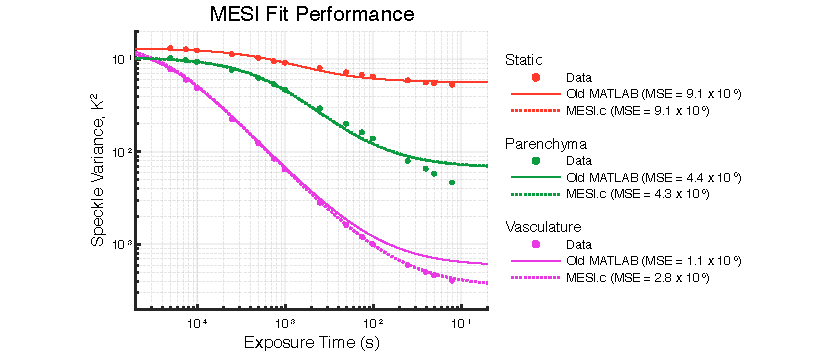
\includegraphics{figures/chapter_4/mesifit.pdf}
    \caption[Comparison of MESI parameter fitting performance for the old MATLAB processing script and the new compiled MESI.c program. ROIs covering vasculature (purple), parenchyma (green), and static skull (orange) were examined. (MSE = Mean Squared Error).]{
        \label{fig:mesifit}
        Comparison of MESI parameter fitting performance for the old MATLAB processing script and the new compiled MESI.c program. ROIs covering vasculature (purple), parenchyma (green), and static skull (orange) were examined. (MSE = Mean Squared Error).
    }
\end{figure}

Figure \ref{fig:mesifit} depicts the resulting fitting performance for the standalone program compared to the original processing script across vascular, parenchyma, and static regions. While there were minimal differences between the mean squared errors of each fit to the original data, the Levenberg-Marquardt algorithm more closely followed the vascular data at longer exposure times compared to the Trust-Region-Reflective algorithm. Regardless of the discrepancies, the enormous increase in computation speed afforded by the MESI.c program makes it the only viable option for large-scale MESI dataset processing.



%%%%%%%%%%%%%%%%%%%%%%%%%%%%%%%%%%%%%%%%%%%%%%%%%%%%%%%%%%%%%%%%%%%%%%%%%%%%%%%
% Section 4.3 - In Vivo Demonstration of MESI
%%%%%%%%%%%%%%%%%%%%%%%%%%%%%%%%%%%%%%%%%%%%%%%%%%%%%%%%%%%%%%%%%%%%%%%%%%%%%%%
\section{\textit{In Vivo} Demonstration of MESI}

The upgraded system was tested \textit{in vivo} with anesthetized mice to demonstrate the MESI technique. Figure \ref{fig:mesidemo}A depicts the 15 speckle contrast images composing a single MESI frame, each acquired with different exposure times. The shorter exposures only reveal the greater flow of the large central vein while the longer exposures show increasing vascular detail. This highlights the sensitivity of an exposure time to only certain ranges of particle speeds and why multiple exposures covering a broad range of values are necessary to more robustly estimate $\tau_c$.

Figure \ref{fig:mesidemo}B depicts the resulting MESI ICT image calculated from the set of speckle contrast images using the process described in Section \ref{sec:mesi_fit}. Because of the large range of $\tau_c$ values, ICT images are typically displayed using a logarithmic scale. This image represents the best estimate of $\tau_c$ currently possible using the LSCI technique. Figure \ref{fig:mesidemo}C plots the speckle variance ($K^2$) of the highlighted vascular and parenchyma regions and their corresponding fits to Equation \ref{eq:mesi}. As $\tau_c$ decreases with increased scattering particle speed, the speckle variance curve shifts towards the left. It is important to sample as much of this curve as possible in order to properly estimate the particle dynamics. The measurements within the vessel would likely benefit from the addition of shorter exposure times since only four exposures (50, 75, 100, 250 $\mu$s) capture the linear portion of the curve.

% Figure - MESI In Vivo Demonstration
\begin{figure}
    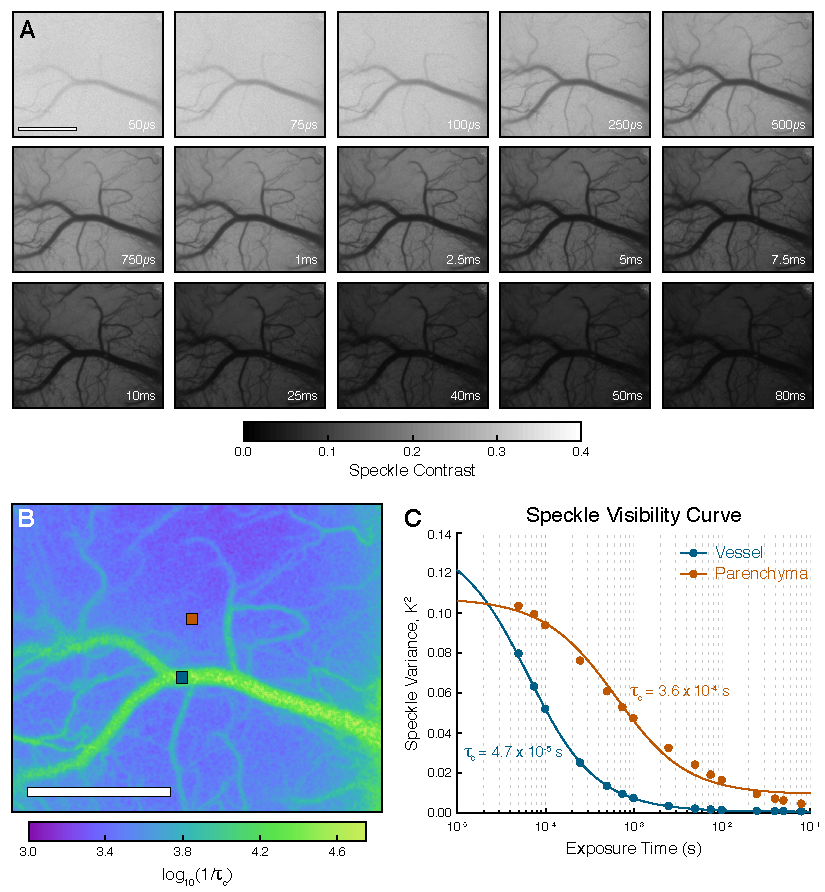
\includegraphics{figures/chapter_4/mesidemo.pdf}
    \caption{
        \label{fig:mesidemo}
        \textbf{(A)} Speckle contrast images from the mouse cortex for each of the 15 MESI exposures and \textbf{(B)} the resulting ICT image. \textbf{(C)} Fitted speckle variance ($K^2$) curves from the vascular (blue) and parenchyma (orange) regions outlined in B (Scale bars = 1 mm).
    }
\end{figure}



%%%%%%%%%%%%%%%%%%%%%%%%%%%%%%%%%%%%%%%%%%%%%%%%%%%%%%%%%%%%%%%%%%%%%%%%%%%%%%%
% Section 4.4 - Sensitivity and Reproducibility of MESI
%%%%%%%%%%%%%%%%%%%%%%%%%%%%%%%%%%%%%%%%%%%%%%%%%%%%%%%%%%%%%%%%%%%%%%%%%%%%%%%
\section{Sensitivity and Reproducibility of MESI}

Microfluidic devices have been used extensively to characterize both LSCI and MESI because they offer controlled testing environments with precise regulation of flow rates \cite{Parthasarathy:2008el, Richards:2013bi, Kazmi:2015du}. While syringe pumps are broadly utilized, they are prone to unwanted oscillations and frequently exhibit slow responsivity to flow changes \cite{Korczyk:2010eu, Zhou:2011ey, Li:2014ca}. Pressure-based flow regulation systems overcome the traditional mechanical limitations of syringe pumps by using air pressure to push fluids at a constant flow rate. Coupled with inline measurements of absolute flow for feedback, these systems allow for users to directly program complex flow profiles.

%%%%%%%%%%%%%%%%%%%%%%%%%%%%%%%%%%%%%%%%%%%%%%%%%%%%%%%%%%%%%%%%%%%%%%%%%%%%%%%
\subsection{Standalone MESI Instrumentation}

The microfluidic tests were performed on a standalone MESI system (Figure \ref{fig:standaloneschematic}) that features similar instrumentation to the previously described dual-modality imaging system. A 785 nm wavelength-stabilized laser diode (300 mW, LD785-SEV300, Thorlabs, Inc.) was mounted in a temperature-controlled housing (TCLDM9, Thorlabs, Inc.) and collimated using an aspheric lens (C280TMD-B, Thorlabs, Inc.). The operating current was set to 380 mA using a laser diode controller (LDC205C, Thorlabs, Inc.) and the diode temperature set to 25 $^\circ$C using a temperature controller (TED200C, Thorlabs, Inc.). The collimated laser light was passed through a free space optical isolator (Electro-Optics Technology, Inc.) to minimize back reflections that interfere with single frequency performance. Because the external volume holographic grating of the stabilized laser diode produces a dark spot in the far field, the laser was coupled into a single mode patch cable (125 $\mu$m cladding, P3-780A-FC-2, Thorlabs, Inc.) to obtain a Gaussian beam. The fiber output was re-collimated (F230APC-780, Thorlabs, Inc.) and modulated using a 100 MHz AOM (3100-125 AOM + 1110AF-AIFO-1.0 RF Driver, Gooch \& Housego) with the first order diffraction isolated and relayed to obliquely illuminate the sample. A pair of camera lenses were used to image the scattered light (AF Nikkor 50mm f/1.8D + AF Micro-Nikkor 105mm f/2.8D, Nikon Corp.) with 2.1x magnification through a bandpass filter (785$\pm$31 nm, 87-773, Edmund Optics Inc.) to a CMOS camera (acA1920-155um, 1920 x 1200 pixels, Basler AG). Only a subset of the overall sensor array was used (1000 x 750 pixels), resulting in a FOV of 2.9 x 2.2 mm. A multifunction I/O device (USB-6363, National Instruments Corp.) was used to produce the camera exposure trigger signals and AOM modulation voltages.

% Figure - Standalone MESI System Schematic
\begin{figure}
    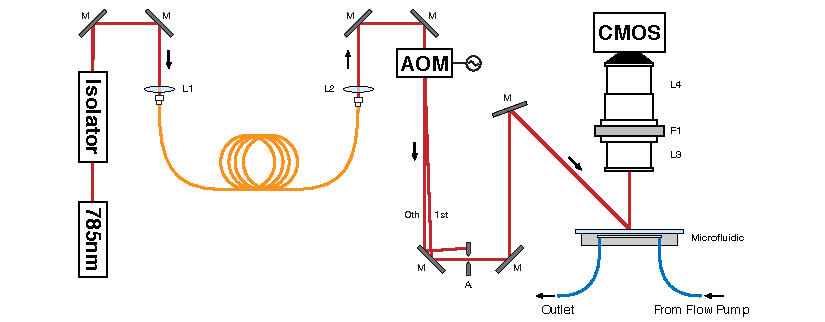
\includegraphics{figures/chapter_4/standaloneschematic.pdf}
    \caption{
        \label{fig:standaloneschematic}
        Schematic of the standalone MESI system used for microfluidic testing.
    }
\end{figure}

%%%%%%%%%%%%%%%%%%%%%%%%%%%%%%%%%%%%%%%%%%%%%%%%%%%%%%%%%%%%%%%%%%%%%%%%%%%%%%%
\subsection{Microfluidic Device}

The microfluidic device utilized for testing MESI featured a single 300 x 300 $\mu$m cross-sectional channel and was fabricated from polydimethylsiloxane (PDMS). 1.8 mg of titanium dioxide (\ce{TiO2}) was added per gram of PDMS to produce background scattering properties ($\mu_s$' = 8 cm$^{-1}$)\cite{Parthasarathy:2008el} similar to that of extravascular brain tissue for visible-NIR wavelengths of light \cite{Yaroslavsky:2002tg}. The complete manufacturing process can be found in \cite{Richards:2016hy}.

In order to measure the flow rate through the phantom, a mass flow sensor (Flow Sensor L, Fluigent Inc.) was placed in-line between the pressure-based flow control system and the inlet of the microfluidic device. The sensor was connected to a proprietary hub (FlowBoard, Fluigent Inc.) and the accompanying software (MAESFLO, Fluigent Inc.) used to record the absolute flow rate. The pressure control system (MFCS-EZ, Fluigent Inc.) was connected to the house air line via a 500 mbar regulator and a 15 mL pressurized reservoir (Fluiwell-1C, Fluigent Inc.) filled with the liquid used in the microfluidic. The flow rate control software was used to adjust air pressure to the reservoir in order to achieve the desired flow rate as measured with the flow sensor. This feedback mechanism allows the flow system to compensate for deviations caused by particle aggregation or air bubbles.

A suspension of 1 $\mu$m diameter polystyrene microspheres (5100A, Thermo Fisher Scientific) in ultra-filtered deionized water was utilized as a blood-mimicking sample. The microsphere concentration was selected to match to the scattering coefficient of whole blood ($\mu_s$ = 243 cm$^{-1}$) assuming a 50\% hematocrit and \ce{SO2} \textgreater 98\% \cite{Yaroslavsky:2002tg}. Prior to a microfluidic experiment, the solution was sonicated in a glass vial to fully suspend the particles and degassed under vacuum to remove any bubbles that could disrupt stable flow. Figure \ref{fig:microfluidic}A depicts a 5 ms LSCI frame of the 300 $\mu$m microfluidic channel with a flow rate of 10 mm/s. The highlighted ROI was used for all MESI ICT measurements. Figure \ref{fig:microfluidic}B depicts the stepped flow profile utilized in all the microfluidic experiments measured using the inline flow sensor. The flow rate was increased from 1-10 mm/s in 0.5 mm/s increments over the course of 40 minutes. This range of flow rates was selected based on prior measurements of red blood cell velocities in rodent microvasculature \cite{Tomita:2008do}.

% Figure - Microfluidic Image + Flow Profile
\begin{figure}
    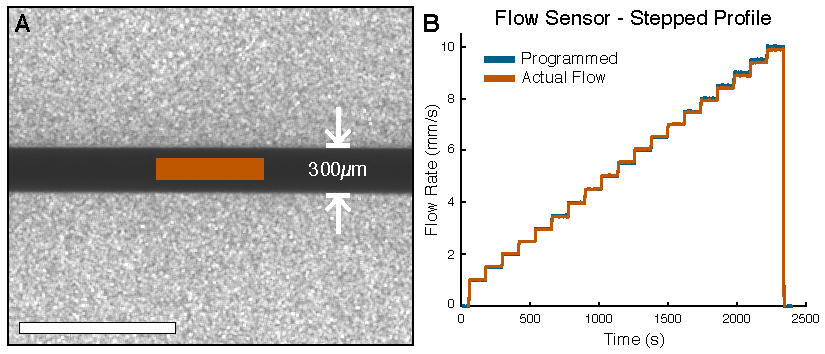
\includegraphics{figures/chapter_4/microfluidic.pdf}
    \caption{
        \label{fig:microfluidic}
        \textbf{(A)} Speckle contrast image of the 300 $\mu$m microfluidic channel (Scale bar = 1 mm). The highlighted ROI is used for all subsequent flow analyses. \textbf{(B)} Programmed flow profile measured using the inline flow sensor with flow rates stepped between 1-10 mm/s.
    }
\end{figure}

%%%%%%%%%%%%%%%%%%%%%%%%%%%%%%%%%%%%%%%%%%%%%%%%%%%%%%%%%%%%%%%%%%%%%%%%%%%%%%%
\subsection{Microfluidic Measurements with MESI}

MESI was used to continuously image the microfluidic channel over the duration of the 40-minute stepped flow profile with an acquisition rate of approximately 1.5 fps. The average speckle contrast was computed at each timepoint within the ROI highlighted in Figure \ref{fig:microfluidic}A. Because $\beta$ is theoretically a constant that only depends upon experimental conditions, it was estimated by performing an initial fit of the median of the data to Equation \ref{eq:mesi}. The full multi-exposure speckle contrast timecourse was then fit to the same equation while holding $\beta$ constant at the estimated value. A moving average filter ($n$ = 5) was applied to the resulting $\tau_c$ timecourse.

In order to compare the fitted values of $\tau_c$ to the absolute measurements from the flow sensor, the relative values of both measurements were computed using the 10 mm/s flow step as the baseline (Figure \ref{fig:microfluidicrelativeflow}A). The MESI rICT measurements closely mirror the flow sensor measurements with increased deviation at the slower flow rates and greater fluctuations over the entire flow profile. The measured speckle variance ($K^2$) and resulting MESI fits for each integer flow rate can be seen in Figure \ref{fig:microfluidicrelativeflow}B. The relationship between increasing flow rates and $\tau_c$ can be seen as the curves shift towards the left. Because $\beta$ was held constant, all the curves are converging to the same value (0.1430) as the exposure time approaches zero. However, this can negatively impact the quality of the resulting fits, as seen with the 1 mm/s curve, which deviates from the measured speckle variance at the shorter exposure times.

% Figure - Microfluidic Relative Flow
\begin{figure}
    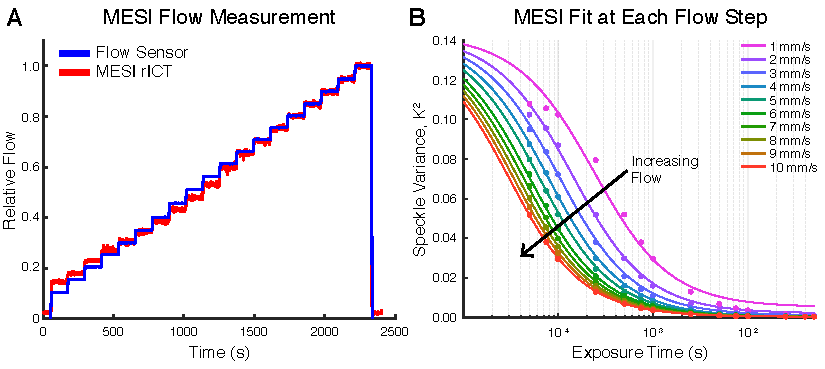
\includegraphics{figures/chapter_4/microfluidicrelativeflow.pdf}
    \caption{
        \label{fig:microfluidicrelativeflow}
        \textbf{(A)} Performance of MESI relative flow estimates compared to the flow sensor. Both measurements were normalized against the final 10 mm/s flow step. \textbf{(B)} Speckle variance curves and MESI fits from each flow step highlighting the relationship between flow rate and $\tau_c$.
    }
\end{figure}

The same measurements were conducted across multiple trials to examine the reproducibility of the MESI estimates of ICT (Figure \ref{fig:microfluidicconsistency}A). Runs 1 and 2 produced almost identical plots while Runs 3 and 4 appear to deviate at flow rates \textgreater 5 mm/s. However, plotting the average ICT against the average flow sensor measurements during each step (Figure \ref{fig:microfluidicconsistency}B) reveals that the flow system overshot the requested values during Runs 3 and 4. Therefore the apparent deviations in ICT seen in Figure \ref{fig:microfluidicconsistency}A were actually caused by the flow rate being higher during those two runs. These results indicate that MESI can provide stable day-to-day estimates of $\tau_c$ across a broad range of flow rates, thereby allowing the parameter to serve as a reliable baseline value for chronic or multiple-animal studies. The strong linear relationship between ICT and absolute flow rate suggests that calibrated measurements could be possible under ideal conditions.

% Figure - Microfluidic Consistency
\begin{figure}
    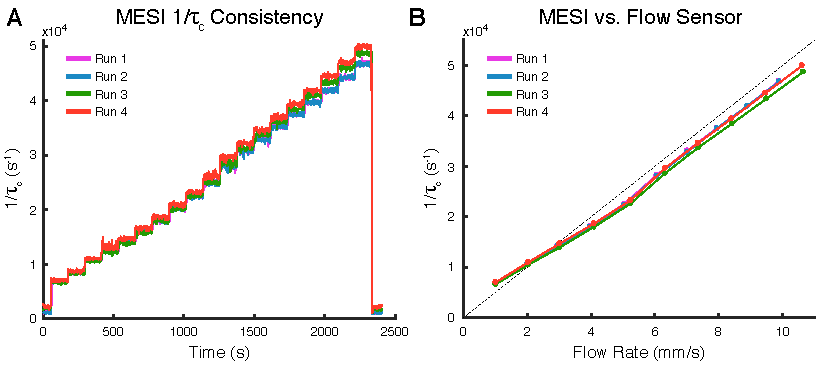
\includegraphics{figures/chapter_4/microfluidicconsistency.pdf}
    \caption{
        \label{fig:microfluidicconsistency}
        \textbf{(A)} Consistency of MESI ICT measurements across multiple trials. \textbf{(B)} MESI underestimates ICT at higher flow rates resulting in a slight divergence from unity. Error bars (s.d.) are displayed but smaller than the data markers.
    }
\end{figure}



%%%%%%%%%%%%%%%%%%%%%%%%%%%%%%%%%%%%%%%%%%%%%%%%%%%%%%%%%%%%%%%%%%%%%%%%%%%%%%%
% Section 4.5 - Discussion
%%%%%%%%%%%%%%%%%%%%%%%%%%%%%%%%%%%%%%%%%%%%%%%%%%%%%%%%%%%%%%%%%%%%%%%%%%%%%%%
\section{Discussion}

The MESI technique allows for more robust estimates of $\tau_c$ compared to traditional single-exposure LSCI \cite{Parthasarathy:2008el}. The improved mathematical model properly accounts for the presence of static scatterers in a sample and the multiple exposure times sample a broader range of flow rates. The implementation of MESI in the dual-modality imaging system facilitates more reliable measurements of flow deficits during targeted photothrombotic stroke \cite{Parthasarathy:2010vo} and improves the quantitative accuracy of chronic CBF measurements \cite{Kazmi:2013hp}. The upgraded system was demonstrated \textit{in vivo} by imaging the cortical vasculature of a mouse and examining the quality of the resulting MESI ICT imagery.

The modifications made to the Speckle Software, optimization of the calibration procedure, and improvements in processing speed have simplified the use of the MESI technique. Because the MATLAB script controlling the camera exposure trigger signals and AOM modulation voltages currently utilizes the ANSI C NI-DAQmx library, integrating the entire MESI calibration and acquisition process into the Speckle Software should be relatively straightforward. The \textgreater800x improvement in processing speed achieved with the compiled fitting program facilitates the full-frame analysis of MESI data that was previously impractical because of computation time. While still insufficient for the real-time processing of full-resolution speckle imagery, downsampling by a factor of two could allow for near 1 fps views of MESI-estimated ICT in the Speckle Software.

The microfluidic measurements conducted on the standalone MESI system further demonstrate the robustness of the technique for estimating $\tau_c$. The linear relationship between ICT and absolute flow rate highlights the broad range of flows that can be properly measured by MESI. The day-to-day stability of ICT estimates allow the metric to serve as a reliable baseline for chronic or multiple-animal studies. While the standalone system utilized an expensive wavelength-stabilized laser diode, any day-to-day fluctuations should be accounted for by the $\beta$ parameter in Equation \ref{eq:mesi} as long as the laser is not mode hopping. The optimization of the LSCI laser diode in the dual-modality system (Section \ref{ssec:laser_stability}) indicated stable speckle contrast measurements over time.



%%%%%%%%%%%%%%%%%%%%%%%%%%%%%%%%%%%%%%%%%%%%%%%%%%%%%%%%%%%%%%%%%%%%%%%%%%%%%%%
% END Chapter 4
%%%%%%%%%%%%%%%%%%%%%%%%%%%%%%%%%%%%%%%%%%%%%%%%%%%%%%%%%%%%%%%%%%%%%%%%%%%%%%%
